
\section{Evaluation}
\label{sec:eval}

This section assesses SafeDE in the context of the aforementioned MPSoC. For that purpose, we synthesized the MPSoC including SafeDE into a Xilinx Kintex UltraScale KCU105 evaluation kit.

\subsection{Functional Validation}
SafeDE implementation in the FPGA is validated with usual VHDL testbenches. To validate its correct operation with representative programs, we have used a bare metal setup and have ported the TACLeBench benchmark suite~\cite{taclebench}. TACLeBench suite is a set of self-contained and open source benchmarks for real-time systems. These benchmarks have their inputs hardcoded along with the source code, thus easing their porting onto a bare metal setup. Their execution times are typically between few hundreds and few millions of cycles, hence easing debugging and the analysis of unexpected results during simulation or emulation. In our evaluation, we use a staggering of 20 cycles ($TH_{stag} = 20$), and recorded the lowest staggering observed during the execution building on the SafeDE statistics register recording this value. Our experiments confirm that the real staggering experienced across all executions of all benchmarks has been never below 20 cycles, therefore confirming the efficacy of SafeDE to preserve a sufficient staggering.

\subsection{Fault injection} 

We have performed a simulation-based fault injection campaign to evaluate the CCF detection capabilities of the aforementioned platform integrating SafeDE. 
We have added non-synthesizable logic into the VHDL files of the CAES Gaisler NOEL-V cores to inject faults in four different locations of the pipeline:

\begin{itemize}
\item \textbf{ALU:} The fault is injected in a random bit, of one of the inputs of one of the two ALUs randomly selected (both the input and the ALU). 
\item \textbf{Late ALU:} Analogous to the previous one, but for late ALUs in the pipeline instead of regular ones.
\item \textbf{Memory:} In the memory stage, the fault is injected in a random bit of the data to be written in the cache.
\item \textbf{Write back:} In the write back stage, the fault is injected in a random bit in a random write port of the register file.
\end{itemize}

In our fault injection campaign, three fault models have been considered: stuck-at-0, stuck-at-1, and bit flip. They set the value of the bit selected for injection to 0, 1 and its logical complementary value respectively. We have enforced the fault during 1 cycle only, but since most of the faults became quickly masked, we have repeated the experiments making faults last 10 cycles instead. In the case of bit flip, we flip the bit and keep such value for 10 cycles regardless of whether the bit is modified.

Since simulations are slow, we have performed our fault injection campaign in one specific benchmark: \texttt{FAC}. In principle, no CCFs should escape SafeDE itself, and we expected to find only CCFs that cannot be detected by light-weight and/or tight lockstepping, regardless of how this is implemented. As shown next, all those insights are already observed with this benchmark.
\texttt{FAC} 
computes the factorial of several numbers and accumulates their results.
The benchmark code is replicated in memory and executed in both cores simultaneously with SafeDE active and imposing a minimum staggering of 20 instructions. 
Faults are injected in a cycle selected randomly in the period where both redundant tasks are active, i.e. since the trail core starts until the head core finishes.
The fault location, namely ALU, late ALU, memory or write back, is randomly selected. The fault is injected in the same location and cycle in both cores to emulate a CCF\footnote{Note, however, that, by having different core states, some faults affecting both cores (e.g., voltage droops) could easily lead to different faults in the cores (e.g., different effects in different locations), hence reducing the probability of a CCF.}. 

We have analyzed the results of each simulation considering the comparison of
results with the golden run outputs, memory dump comparison, and monitoring the AHB transmission during the simulation (to check for invalid memory accesses).

The possible outcomes considered are based on the categories in \cite{FaultModel}, which we extend conveniently to consider additional categories relevant for CCFs:
\begin{itemize}
 \item \textbf{Timeout:}  The simulation exceeds 90 seconds. Note that the fault-free simulation takes 35 seconds.
 \item \textbf{Crash:}  The simulation process is terminated abnormally.
 \item \textbf{Software detected:} Error detected by software comparison between the results of both cores, including differences across data in memory.
 \item \textbf{Identical memory SDC:} Both executions produce the same memory corruptions (SDC). They are identified in the post-analysis using the memory dumps.
 \item \textbf{DUE:}  One of the cores wrote outside its memory limits causing a non recoverable error. It is detected with the AHB transaction monitoring.
 \item \textbf{Masked:}  Outputs were identical to the golden run outputs, including memory dumps and AHB transmissions. 
 \item \textbf{Undetected error:}  The software comparison did not raise any error but the result is different from the golden run.
\end{itemize}

Note that, only \emph{undetected error} and \emph{identical memory SDC} categories correspond to CCFs.

\begin{table}[t!]
  \caption{Fault injection results classified by fault model.}
  \label{fault_injection_results}
  \centering
  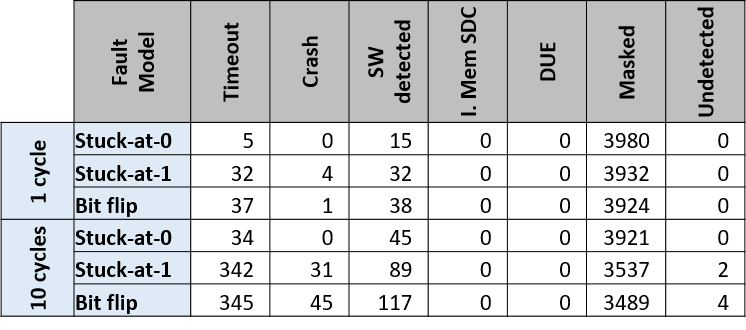
\includegraphics[width=1\columnwidth]{imgs/faultinjection2.png} 
  \end{table}

Table~\ref{fault_injection_results} summarizes the fault injection results. For each fault model and fault duration (either 1 or 10 cycles), we performed 4,000 simulations. 
As shown, out of the 24,000 simulations performed, some simulations led to \emph{timeout} or \emph{crash}, hence making the error easily detectable. The number of such cases is higher for a larger fault duration. Some other faults led to errors detected by comparing the outputs, including data in memory (\emph{SW detected}). 
Some simulations produced errors in memory, but none of those cases had the two memory dumps equal. Hence, \emph{identical memory SDC} -- one of the two CCF categories -- is always zero.
During the injection campaign, no DUE appeared. Still, some injections that were classified in the timeout, crash or error detected categories also wrote out of their memory limits. 
Most of the faults injected were masked. This is particularly true if the fault duration is short (1 cycle).
Finally, only in six of the simulations the error produced could not be detected by the software comparison. In all occasions, the faults were injected in the write back stage. Since these six experiments would correspond to a CCF despite using lockstepping, we analyze them in detail.

The benchmark \texttt{FAC} calculates and accumulates the factorials of the numbers from 12 to 0 using recursion. As shown in Figure~\ref{fig:fac_dump}, the assembly code obtained after compilation has three main sections: initialization, an outer loop to accumulate the factorials and an inner loop to derive the factorials. 
The fault injected (a bit flip) in the head core is applied while the factorial of 8 is being processed in the inner loop. The least significant bit of the second write port of the register file becomes 1 instead of 0, and the value store is erroneous for up to 10 cycles. 
However, those values are read through a bypass in the inner loop instead of from the register file, so no impact is observed in the inner loop. 
In the last iteration of the inner loop, the result of the factorial is stored in register \texttt{a4} (line 8) with an erroneous value (due to the duration of the fault). Later, the register \texttt{a4} is read as an operand for \texttt{addw} instruction in line 17, which accumulates all the calculated factorials. Therefore, this error is propagated to the output. Particularly, the erroneous result contains one bit flip in the least significant bit with respect to the correct result.

\begin{figure}[t!]
\centering
  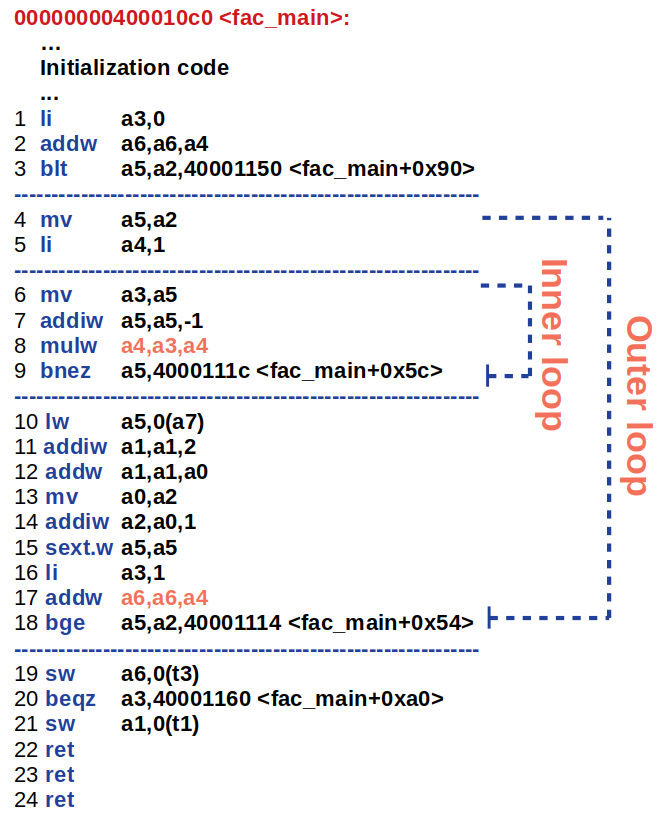
\includegraphics[width=0.85\columnwidth]{imgs/fac_assembly.png} 
  \caption{Excerpt of the assembly code of the benchmark \texttt{FAC}.}
  \label{fig:fac_dump}
\end{figure}


In the trail core, the fault is injected while the core is executing the outer loop. The fault affects several instructions, but all the errors except one are masked because they are either overwritten or not read since they are forwarded like in the head core. The error not masked is produced in line 17 when the result of the addition is written back to the \texttt{a6} register, which stores the accumulation of the factorials. Again, the final value contains one bit flip with respect to the correct output in the least significant bit. 
Therefore, even though the fault affects both cores differently, in the end, it produces the same bit flip in the accumulated register (\texttt{a6}), which stores the output value. Thus, the software is not capable of detecting the error, not because of a malfunctioning of SafeDE, but because of the semantics of the benchmark \texttt{FAC}. 
In fact, even if we used tight lockstepping, external core activity would be identical for both cores and no error would be detected.

We content that, despite we could produce this apparent CCF in our fault injection campaign, such effect would be very unlikely to occur in practice since both cores have different states when the fault occurs, and this should lead to heterogeneous electric impact, hence causing heterogeneous errors (e.g., affecting only one core, or affecting different bits or locations of both cores).

\subsection{Execution time overhead}

We have measured the performance of the TACLeBench in three different scenarios: (1) \emph{Isolation}, where only one core runs the benchmark; (2) \emph{Redundancy without diversity}, where two cores run the benchmark without enforcing any staggering; and (3) \emph{Redundancy with diversity} enforced by SafeDE with $TH_{stag} = 20$.
Such $TH_{stag}$ is set large enough so that both cores cannot hold any common instruction in their pipelines to avoid a case where such instruction causes all the activity and hence, a CCF is possible. Since the pipeline has 7 stages, and each stage can hold up to 2 instructions, any value above 14 suffices to guarantee that instructions executed across cores at any time differ.

To discount the effect of effects such as DRAM refreshes and other minor performance variations, we run each benchmark 1,000 times and report average cycle counts. In any case, variations observed are up to few tens of cycles across runs.

\begin{figure}[t!]
\centering
  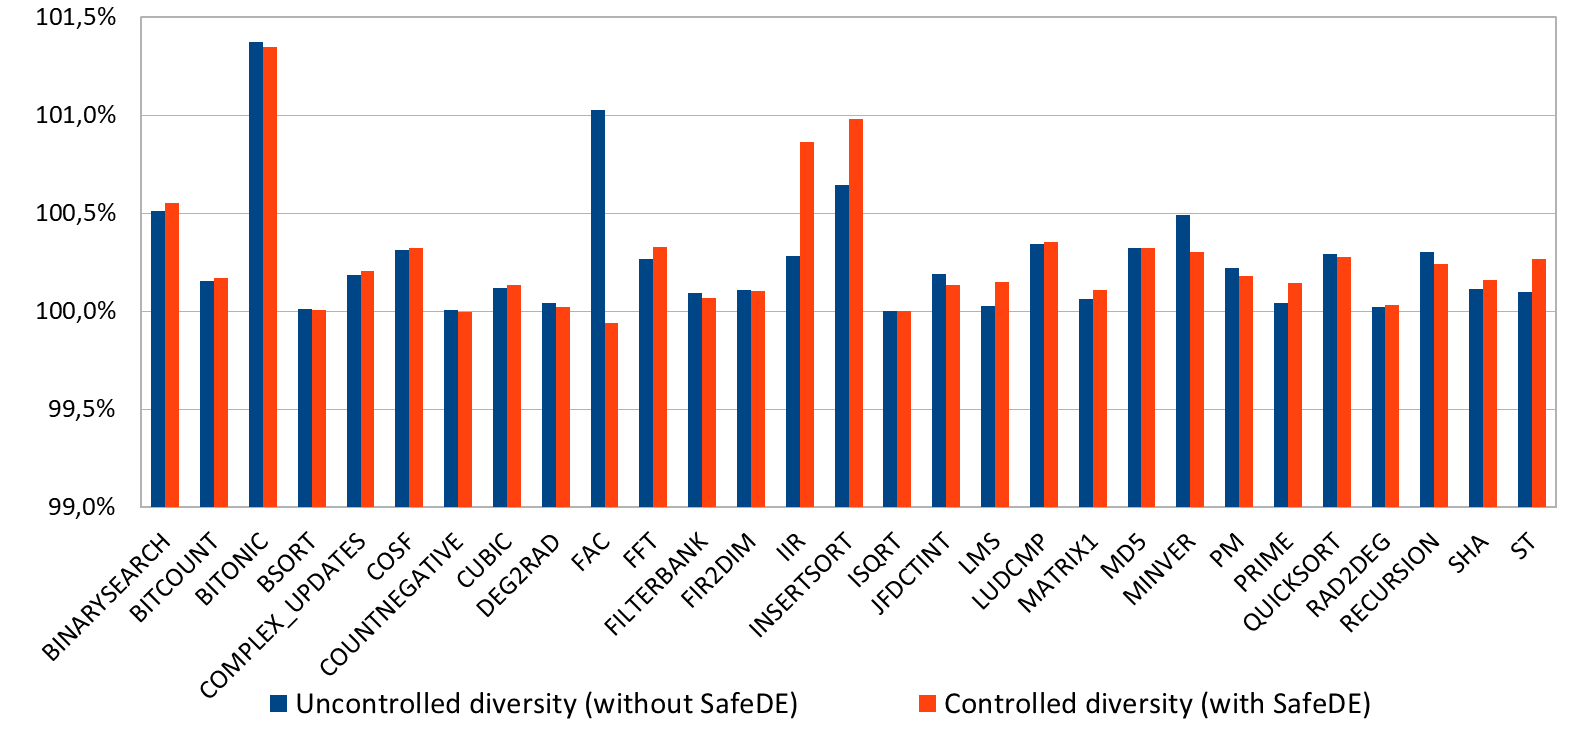
\includegraphics[width=1\columnwidth]{imgs/tacle_results.png} 
  \caption{Average execution time of different TACLeBench benchmarks normalized w.r.t. their execution time in isolation.}
  \label{fig:tacle_results}
\end{figure}

As shown in Figure~\ref{fig:tacle_results}, performance degrades only by 0.3\% on average (up to 1.3\% for \texttt{BITONIC}) w.r.t. isolation runs, and 0.003\%, so $\approx$0\% (up to 0.6\% for \texttt{IIR}) w.r.t. redundancy without diversity.
Performance variations across runs, and even marginal performance gains with SafeDE relate to the initial state of the branch predictor, and to memory alignment of the binaries impacting the instruction cache behavior, since in the case of SafeDE we execute additional instructions to configure SafeDE. The relative effect of those variations can be larger for short programs, as it is the case for \texttt{FAC}, with variations in the range of 1\%. In fact, those variations have a higher impact than the tiny performance degradation of SafeDE w.r.t. redundancy without diversity.

Overall, performance overheads are tiny due the very low staggering threshold needed by SafeDE (20 cycles in our case), which is far lower than that for the software-only solution (e.g., 100$\mu$s or more)~\cite{SergiDFT}.

\subsection{Hardware costs}

We have used the Vivado 2018.1 Toolchain to synthesize our MPSoC for the Xilinx UltraScale KCU105 FPGA. SafeDE required 261 LUTs and 417 registers, whereas the whole SoC required approximately 114,000 LUTs and 74,000 registers, and each core individually 38,000 LUTs and 17,000 registers. Hence, SafeDE has negligible hardware costs (0.23\% of the LUTs and 0.56\% of the registers of the entire SoC). Those results could be further improved by dropping the statistics additions of SafeDE.
